\section{Injuries and Diseases, with Examples In Each Sign: What Injuries and Diseases are Caused by Aries and the Succeeding Signs (36K,37P)}

Since the old astrologers have written about the topic of injuries very obscurely, we will lucidly explain it. Some astrologers, with reference to the underlying parts of the body and the mind, for each nativity \textbf{/104P/} have <assigned> the limbs starting with the Lot of Fortune and with Daimon, and they make their forecasts concerning injuries and diseases with reference to the proximity of malefics. For
example:

% NOTE: had to add extra column at beginning as first heading
%		  was not being made bold
%
\begin{table}[ht]
\begin{footnotesize}
\begin{center}
\caption{Limbs from the Lot of Fortune}
\label{Table 2.2}
\vspace{0.5cm}
\begin{tabular}{lllll}
\toprule
\multirow{2}{*}
	& \textbf{Sign} & \textbf{Part} & \textbf{Sign} 
		& \textbf{Part}\\ 
	& & \textbf{Affected} &  & \textbf{Affected} \\
\hline
& The Lot of Fortune & breast & Sign 7 & knees \\
& Sign 2 & flanks & Sign 8 & calves \\
& Sign 3 & belly & Sign 9 & feet \\
& Sign 4 & groin & Sign 10 & head \\
& Sign 5 & genitals & Sign 11 & face, neck \\
& Sign 6 & thighs & Sign 12 & \parbox[t]{2cm}{arms, 
\\shoulders} \\
\bottomrule
\end{tabular}
\end{center}
\end{footnotesize}
\end{table}

\newpage
Diseases are counted from Daimon: \\
\begin{table}[hbt!]
\begin{footnotesize}
\begin{center}
\caption{Diseased Body Part from the Daimon}
\label{Table 2.3}
\vspace{0.5cm}
\begin{tabular}{lllll}
\toprule
\multirow{2}{*}
	& \textbf{Sign} & \textbf{Part} & \textbf{Sign} 
		& \textbf{Part}\\ 
	& & \textbf{Affected} &  & \textbf{Affected} \\
\hline
& Daimon & heart & Sign 7 & bladder \\
& Sign 2 & stomach & Sign 8 & bowels \\
& Sign 3 & \parbox[t]{2.5cm}{kidney, sperm \\ ducts} 
       & Sign 9 & \parbox[t]{2.5cm}{brain, teeth,\\ ears} \\
& Sign 4 & colon & Sign 10 & gullet \\
& Sign 5 & liver & Sign 11 & tongue \\
& Sign 6 & intestines & Sign 12 & stomach \\
\bottomrule
\end{tabular}
\end{center}
\end{footnotesize}
\end{table}

This becomes obvious if one begins with \Leo\xspace and \Cancer, then goes in order, since the \Moon\xspace <\Cancer> is the Fortune of the Universe, and the \Sun\xspace <\Leo> is Mind and Divinity.

\subsection{\textit{[Indications from Signs]}}
That is what the earlier astrologers stated. The following seems more accurate in our experience: 

Aries \mn{\Aries} is indicative of the head in general, the sensory faculties, and the eyesight. In the point now at issue, \Aries\xspace causes headaches, dimming of vision, strokes, deafness, blindness, leprosy, lichenous scaliness of the skin, loss of hair, mange, baldness, stupor, festering sores, sudden attacks of panting, arthritic joints, tumors, plus whatever syndromes occur of the sensory faculties, the ears, and the teeth.

Taurus \mn{\Taurus} is indicative of the neck, face, gullet, eyebrows, and nose. This sign causes hunchback because
of its round-shouldered appearance and lameness because of its bent hoof; \textbf{/110K/} also pains and dangerous crises of the eyes and blindness because of the Pleiades. This is a sneaky and degraded sign. It causes fits, excision of the uvula, carbuncles, goiter, choking, as well as injuries, diseases, and pains of the nostrils, falls from high places or from animals, fractures of the limbs, throat tumors, mutilation, sciatica, abscesses.

Gemini \mn{\Gemini} is indicative of shoulders, arms, hands, fingers, joints, sinews, strength, courage, change, the
birth of women, speech, mouth, blood vessels, the voice. When afflicted, \Gemini\xspace causes injuries to these parts; it also brings attacks of bandits and enemies accompanied by wounds, cuts, and loss of limbs. It brings jaundice and falls from high places.

Cancer \mn{\Cancer} is indicative of the chest, stomach, breasts, spleen, mouth, the hidden parts, the dimming of vision and blindness because of the nebula <in \Cancer>. Under this sign the following occur: leprosy,
lichenous scaliness of the skin and of the face, strokes, dropsy arising from complaints of the spleen, staggering gait, bilious syndromes, \textbf{/105P/} lameness, jaundice, piebald skin, buck teeth, crossed eyes, loss of eyelashes, diseased eyelids, twisted spines, injuries from aquatic animals, birthmarks and moles around the eyes, coughs bringing up blood, jaundice, pleurisy, and lung ailments.

Leo \mn{\Leo} is indicative of the flanks, the loin, the heart, courage, vision, sinews. Under this sign the
following occur: lunacy or superstitious terrors, convulsions/wounds caused by violence or vice, or resulting from bravery or asceticism, loss of limbs, amputation, injury to the eyes. It is also the cause of foul odors. It also causes ugliness, amputations, fractures, falls from high places or from animals, bites from wild beasts, and injuries from buildings collapsing and from burns, as well as depression, cancer, and
homosexuality.

Virgo \mn{\Virgo} is indicative of the belly, the internal organs, and the internal reproductive organs. It causes attacks of passion; with respect to intercourse, it makes people who are either weak, or strong and chaste.
(So that we may not seem too lengthy—the injuries and diseases caused by a sign or star are obvious from the nature of the sign and the star.) Virgo causes orthopnoea, hernia, superstitious terrors; in women it causes hysterical syndromes and complaints of the womb.

Libra \mn{\Libra} is indicative of the hips, buttocks, the colon, the genitals, the hind parts. This sign causes
paralysis, hernia, rupture, dysentery, dropsy, kidney stones.

Scorpio \mn{\Scorpio} is indicative of the genitals and the rump. Because of its sting, it causes dimming of vision, blindness, weak eyesight, kidney stones, strangury, recurrent illness, hernia/promiscuity <?>, fistula.

Sagittarius \mn{\Sagittarius} is indicative of the thighs \textbf{/111K/} and the groin. Under this sign occur piebald skin with birthmarks, baldness, weak vision, eyestrain or blindness, bad breath, gout. It also causes falls from high
places or from beasts, the loss of limbs and injuries from wild animals, and births with extra limbs.

Capricorn \mn{\Capricorn} is indicative of the knees, the sinews, and internal and external sprains and strains because of its mysterious character. It causes weak vision and blindness because of its spiny vertebrae. It causes insanity, troubles from moist things; also delirium, incestuous women, lesbians and nymphomaniacs, banditry, and vice.

Aquarius \mn{\Aquarius} is indicative of the legs, calves, sinews, and joints. It causes elephantiasis, jaundice, a sallow color, lameness, dropsy, insanity, castration, fractures, and sometimes strangury.

Pisces \mn{\Pisces} is indicative of the feet, the sinews, and the toes. Under it occur arthritis, lichenous scaliness of the skin and leprosy, and people who are on the way down, reviled and suffering many injuries. \Pisces\xspace causes births with extra limbs, halting speech, deafness, mange, wounds from aquatic beasts, or affliction from moist syndromes.

All this being given, it will be necessary to examine each nativity closely to see \textbf{/106P/} in which sign the Lot of Fortune is located, for the nature of the sign will indicate the injury. The ruler of the Lot of Fortune will be particularly indicative, along with the sign in which it is located. 

Likewise examine Daimon and its ruler to see in which sign they are located, for these will clarify <the nature of> the disease.

The stars in the Place of Occupation\footnote{The 10th house.} must be examined by you in the same way. Injuries and diseases will be quite violent if malefics are in conjunction or in aspect with these places or their houserulers. The native will be hale and healthy whenever the places and their rulers are favorably situated and not afflicted.

Each star has its own effect according to its allotted nature: if—to take a hypothetical example—the Lot is in Aries and its ruler, \Mars, is also there (since \Mars\xspace rules \Aries\xspace and \Scorpio), you can foretell an injury
to the head and the genitals or the rump. Whatever the star should cause, judging from its nature, it will cause. 

Occasionally, if both places are afflicted, injuries and diseases occur, especially when malefics rule or
are in aspect. 
\newpage
% --------------------------------------------------------1-
\subsection{\textit{[Examples]}}
\subsubsection{\textit{[Chart 20: Blind, qouty]}}
For example—so that we will not seem to talk in riddles—<take the following nativity>: \Sun, \Jupiter,
\Mars\xspace in \Capricorn, \Moon, Ascendant in \Leo, \Saturn\xspace in \Taurus, \Venus, \Mercury\xspace in \Aquarius, the Lot of Fortune <in \Capricorn>, the ruler of Fortune, \Saturn, in \Taurus
\footnote{\textit{Greek Horoscopes} dates the chart (L87) to approximately January 9, 87 AD (p.95)}.

\clearpage
\begin{wrapfigure}[14]{R}{7cm}
\centering
\vspace{-20pt}
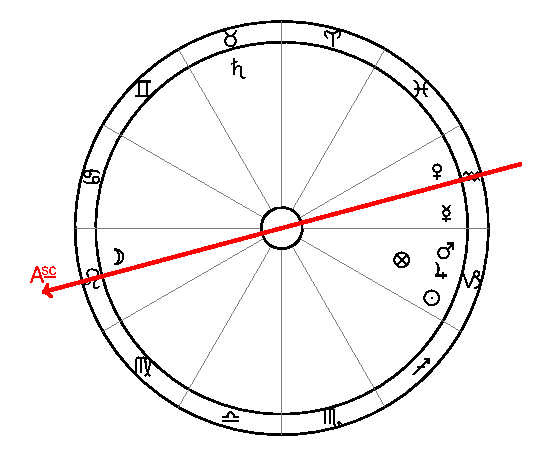
\includegraphics[width=0.68\textwidth]{charts/2_36_1}
\caption{Chart 20 [II.36.1, GH L87]}
\label{fig:chart20}
\end{wrapfigure}

The native was blind on account of the Pleiades and because of the malefic \Saturn, and he had unmentionable \textbf{/112K/} vices because of both signs <\Capricorn, \Taurus>. In addition, \Jupiter, the ruler of Daimon (in \Pisces), was found in \Capricorn. From these configurations it was clear that he had gout. The Lot and its ruler was sufficient to reveal the disease and the injury.
\newpage

% -- Chart 21 ---------------------------------------------2-
\subsubsection{\textit{[Chart 21: Bald, blind]}}
Another example: \Sun, \Venus, \Mars\xspace in \Sagittarius, \Moon\xspace in \Libra, \Saturn\xspace in \Cancer <error for
\Gemini>, \Jupiter\xspace in \Virgo, \Mercury\xspace in \Scorpio, Ascendant in \Capricorn, the Lot in \Scorpio
\footnote{\textit{Greek Horoscopes} dates the chart (L118) to approximately November 26, 118 AD (p.114) This chart is also used as an example in Book VII, sections 2 and 6.}.

\clearpage
\begin{wrapfigure}[14]{R}{7cm}
\centering
\vspace{-20pt}
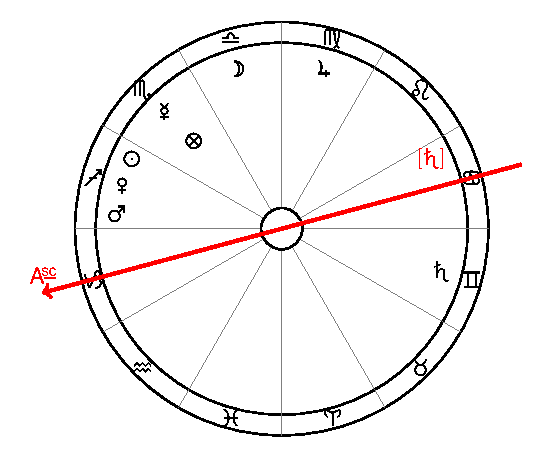
\includegraphics[width=0.68\textwidth]{charts/2_36_2}
\caption{Chart 21 [II.36.2, GH L118]}
\label{fig:chart21}
\end{wrapfigure}

The genitals were injured because the ruler of \Scorpio\xspace <\Mars> was in \Sagittarius. The native was bald and blind on account of <\Sagittarius’> arrow. \Jupiter, the ruler of Daimon <\Pisces>, was found in <the IX Place of>
the God and caused him to recover his sight with the help of the god. He became a seer.

% -- General notes ----------------------------------------
\subsubsection{\textit{[General Delineation Notes]}}
So we see that benefics unfavorably situated are perverted\mnbm and lead to infirmities and diseases, while malefics favorably situated cause no infirmities, just temporary and intermittent bouts of illness. 

If the rulers of the Lot of Fortune or of Daimon happen to be in <the IX Place of> the God or <the III Place of>
the Goddess and are intercepted\mn{Interception} or aspected by malefics, they cause men to be struck dumb, to be raving lunatics, or to be seers. As the Compiler says, and most reasonably too: “If the star which indicates infirmity is in a Potent Place\mn{Potent Place} and \textbf{/107P/} is beheld by a malefic, the disease which befalls will be incurable and untreatable. If a benefic is in conjunction or in aspect with the Harmful Place, the native will be cured by medicine or by the help of a god.” (By “Potent Place” he means the angles and the two <Places> which rise just after <the angles>, especially when the malefics which hold <the rulership> are in these places.) 

It is necessary to scrutinize accurately the degree-position of the Lots, because often a rough calculation puts the Lot in one sign, but an exact calculation puts it in another. This frequently happens as a result of the positions of the luminaries or of the Ascendant, if they are found either at the beginning or the end of a sign. 

Generally speaking, the \Sun, the \Moon, \Saturn, and \Mercury, when in opposition or when rising just after <another star>, bring injuries to the eyes and onsets of other disease, insanity, or strokes. 

The \Sun\xspace rising just after \Mars\xspace or located in the same sign causes coughing or spitting blood and heart trouble, as well as injuries to the vision. 

\Saturn\xspace and \Mars\xspace at IC either together or alone make men of poor vision and subject to sudden fits, men who see visions of the gods or the dead, men who are initiated into secret, mystic lore. The same stars, if they are in opposition or in superior aspect with the new or full moon, or if the individually behold the \Moon\xspace while the moon is passing out of a given phase, \textbf{/113K/} cause lunacy,
possession, fits, and can strike men dumb.

\newpage
% -- Chart 22 ---------------------------------------------3-
\subsubsection{\textit{[Chart 22: Tender feet, a lunatic]}}
For example: \Sun, \Saturn\xspace in \Capricorn, \Moon\xspace in \Scorpio, \Jupiter\xspace in \Leo, \Mars\xspace in \Pisces, \Venus, \Mercury\xspace in \Aquarius, Ascendant in \Virgo, the Lot of Fortune in \Scorpio, Daimon in \Cancer
\footnote{\textit{Greek Horoscopes} dates the chart (L106) to approximately January 16, 106 AD (p.103).}.

\clearpage
\begin{wrapfigure}[14]{R}{7cm}
\centering
\vspace{-30pt}
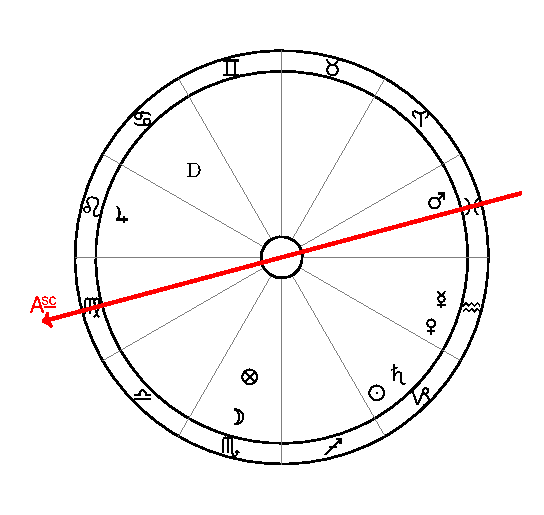
\includegraphics[width=0.68\textwidth]{charts/2_36_3}
\caption{Chart 22 [II.36.3, GH L106]}
\label{fig:chart22}
\end{wrapfigure}

\noindent \Saturn was in opposition to Daimon, which influences the intellectual and spiritual qualities, and \Saturn\xspace beheld the full moon, which was the immediately preceding phase. The ruler of the Lot of Fortune <\Mars> was in opposition to the Ascendant. The native had an injury in the fated places, tender feet, and—most significantly—he was a lunatic. 

\newpage
% -- Chart 23 ---------------------------------------------4-
\subsubsection{\textit{[Chart 23: Visions]}}
Another example: \Sun\xspace in \Sagittarius, \Moon\xspace in \Cancer, \Saturn\xspace in \Taurus, \Jupiter, \Mercury\xspace in \Scorpio, \Mars\xspace in \Leo, \Venus\xspace in \Capricorn, Ascendant in \Aquarius, the Lot of Fortune in \Leo <!should be \Virgo>
\footnote{\textit{Greek Horoscopes} dates the chart (L85) to approximately November 24, 85 AD (p.94).}.

\clearpage
\begin{wrapfigure}[14]{R}{7cm}
\centering
\vspace{-20pt}
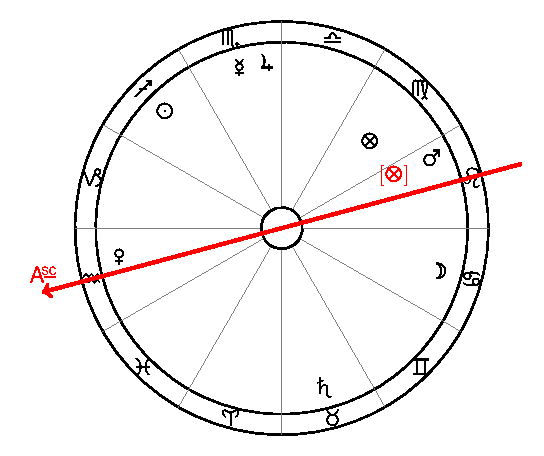
\includegraphics[width=0.68\textwidth]{charts/2_36_4}
\caption{Chart 23 [II.36.4, GH L85]}
\label{fig:chart23}
\end{wrapfigure}

\noindent \Mars\xspace is there, and \Saturn in superior aspect. The \Sun, found in the places of \Jupiter, is indicative of things the ruler of the sinews. Since \Saturn\xspace was found at IC, the native had visions of the gods and of the dead.

\newpage
\clearpage
% -- Chart 24 --------------------------------------------5-
\subsubsection{\textit{[Chart 24: Homosexual]}}
Another example: \Sun\xspace in \Aquarius, \Moon\xspace in \Virgo, \Saturn\xspace in \Taurus, \Jupiter, \textbf{/108P/} Ascendant in \Gemini, \Mars\xspace in \Cancer, \Venus\xspace in \Pisces, \Mercury\xspace in \Capricorn, the Lot of Fortune in \Capricorn, Daimon in \Scorpio
\footnote{\textit{Greek Horoscopes} dates the chart (L116) to approximately January 21, 116 AD (p.112).}.

\clearpage
\begin{wrapfigure}[13]{R}{7cm}
\centering
\vspace{-30pt}
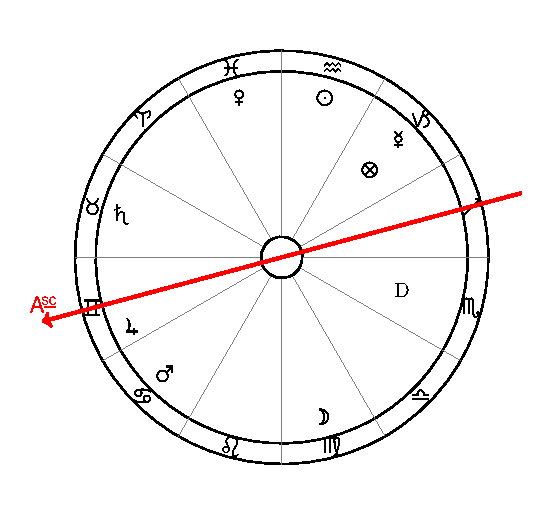
\includegraphics[width=0.68\textwidth]{charts/2_36_5}
\caption{Chart 24 [II.36.5, GH L116]}
\label{fig:chart24}
\end{wrapfigure}

\noindent Malefics were in opposition to the Lots. The native was homosexual and had unmentionable vices, because \Capricorn\xspace is a lewd sign and its ruler <\Saturn> was in \Taurus, a pathic sign. \Scorpio\xspace also indicates this kind of vice.

\newpage
% -- Chart 25 --------------------------------------------6--
\subsubsection{\textit{[Chart 25: Castration]}}
Another example: \Sun, \Venus\xspace in \Sagittarius, \Moon\xspace in \Cancer, \Saturn\xspace in \Gemini, \Jupiter, \Mars\xspace in \Leo, \Mercury\xspace in \Scorpio, Ascendant in \Capricorn, the Lot of Fortune in \Leo, Daimon in \Gemini
\footnote{\textit{Greek Horoscopes} dates the chart (L117) to approximately November 30, 117 AD (p.114)}. 

\clearpage
\begin{wrapfigure}[14]{R}{7cm}
\centering
\vspace{-20pt}
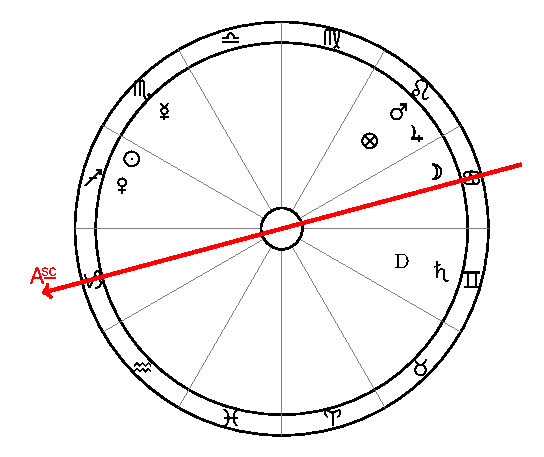
\includegraphics[width=0.68\textwidth]{charts/2_36_6}
\caption{Chart 25 [II.36.6, GH L117]}
\label{fig:chart25}
\end{wrapfigure}

\noindent \Saturn\xspace located in this sign caused him to be castrated. The ruler <of \Gemini>, \Mercury, was in \Scorpio, which indicated the genitals, and the \Sun\xspace in \Sagittarius\xspace indicated the region of the groin\ldots
\ldots Malefics entering Daimon or in opposition <to Daimon> cause insanity and possession\ldots

\newpage
% -- Chart 26 ---------------------------------------------7-
\subsubsection{\textit{[Chart 26: Blind]}}
Another example: \Sun, \Moon, \Mercury, Ascendant in \Scorpio, \Saturn\xspace in \Leo, \Jupiter\xspace in \Cancer, \Mars\xspace in \Capricorn, \Venus\xspace in \Libra, the Lots in \Scorpio
\footnote{\textit{Greek Horoscopes} dates the chart (L92) to approximately November 17, 92 AD (p.97)}. 

\clearpage
\begin{wrapfigure}[13]{R}{7cm}
\centering
\vspace{-20pt}
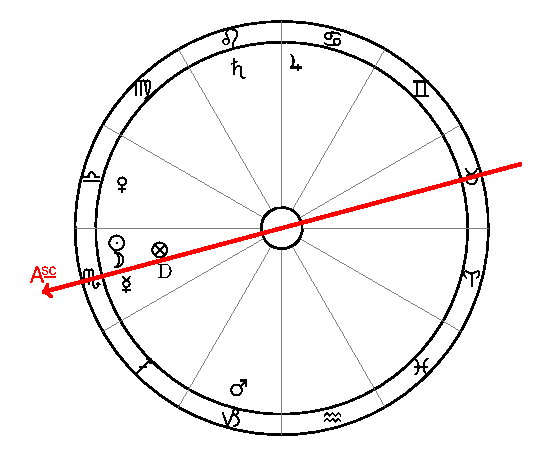
\includegraphics[width=0.68\textwidth]{charts/2_36_7}
\caption{Chart 26 [II.36.7, GH L92]}
\label{fig:chart26}
\end{wrapfigure}

The native was blind because of <\Scorpio’s> sting. In
addition \Saturn\xspace was in superior aspect to the new \Moon\xspace <in \Scorpio> and to the luminaries, and the ruler <of \Scorpio>, \Mars, was unfavorably situated.
\newpage

% -- Chart 27 ---------------------------------------------8-
\subsubsection{\textit{[Chart 27: Leprosy, mange ]}}
\textbf{/114K/} Another example: \Sun, \Mercury\xspace in \Taurus, \Moon\xspace in \Aquarius, \Saturn, \Venus\xspace in \Aries, \Jupiter\xspace in \Virgo, \Mars\xspace in \Pisces, Ascendant in \Leo, the Lot of Fortune in \Taurus. Its ruler, \Venus, was in \Aries\xspace with \Saturn
\footnote{\textit{Greek Horoscopes} dates the chart (L83) to approximately April 28, 83 AD (see also section 21.4) (p.93)}. 

\clearpage
\begin{wrapfigure}[10]{R}{7cm}
\centering
\vspace{-20pt}
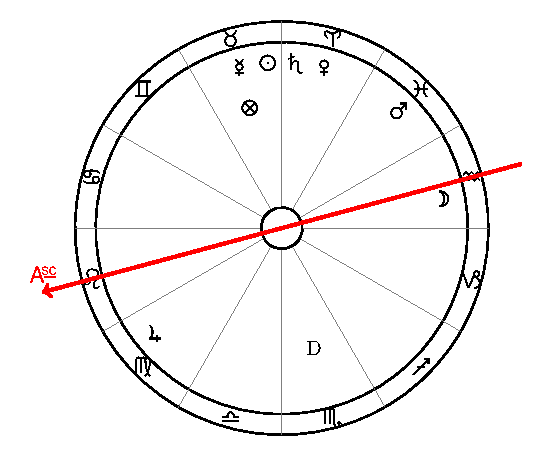
\includegraphics[width=0.68\textwidth]{charts/2_36_8}
\caption{Chart 27 [II.36.8, GH L83]}
\label{fig:chart27}
\end{wrapfigure}

The native had mange on the head and leprosy and lichenous scaliness of the skin because the ruler <\Mars> of Daimon <in \Scorpio> was in \Pisces.

\newpage
% -- Chart 28 ---------------------------------------------9-
\subsubsection{\textit{[Chart 28: Abnormally short arms ]}}
Another example: \Sun, \Mars\xspace in \Taurus, \Moon\xspace in \Virgo, \Saturn\xspace in \Sagittarius, \Jupiter\xspace in \Gemini, \Mercury, \Venus, Ascendant in \Aries, the Lot of Fortune in \Sagittarius with its ruler <\Jupiter> in \Gemini
\footnote{\textit{Greek Horoscopes} dates the chart (L104) to approximately April 23, 104 AD (p.102).}.

\clearpage
\begin{wrapfigure}[6]{R}{7cm}
\centering
\vspace{-20pt}
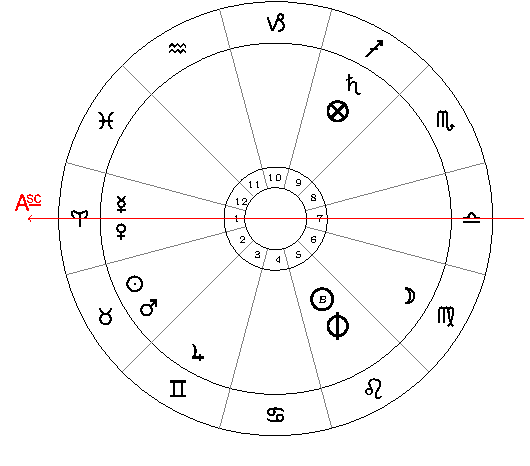
\includegraphics[width=0.68\textwidth]{charts/2_36_9}
\caption{Chart 28 [II.36.9, GH L104]}
\label{fig:chart28}
\end{wrapfigure}

Furthermore Daimon was in \Leo\xspace and its ruler <\Sun> was in \Taurus. The native had abnormally short arms.

\newpage
% -- Chart 29 --------------------------------------------10-
\subsubsection{\textit{[Chart 29: Insane ]}}
Another example: \Sun, \Mercury\xspace in \Aries, \Moon\xspace in \Pisces, \Saturn, Ascendant in \Aquarius, \Mars, \Venus\xspace in \Taurus, \Jupiter\xspace in \Libra, the Lot of Fortune in \Pisces, the Lot of Daimon in \Capricorn
\footnote{\textit{Greek Horoscopes} dates the chart (L108) to approximately March 28, 108AD (p.104)}.

\clearpage
\begin{wrapfigure}[13]{R}{7cm}
\centering
\vspace{-20pt}
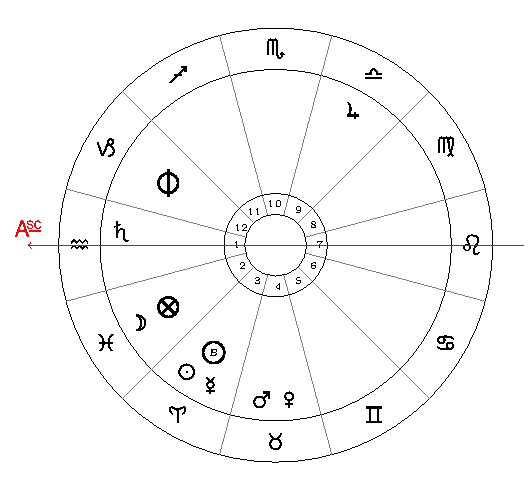
\includegraphics[width=0.68\textwidth]{charts/2_36_10}
\caption{Chart 29 [II.36.10, GH L108]}
\label{fig:chart29}
\end{wrapfigure}

The native was possessed of a god and insane. The ruler, \Jupiter, of the Lot of Fortune was found in \Libra, the
IX Place of the God, and the ruler of Daimon, \Saturn, was in the Ascendant. \Venus\xspace was found at IC.

\newpage
% -- Chart 30 --------------------------------------------11-
\subsubsection{\textit{[Chart 30: Hunchback ]}}
Another example: \Sun, \Mercury\xspace in \Leo, \Moon\xspace in \Scorpio, \Saturn, Ascendant in \Aries, \Jupiter\xspace in \Pisces, \Mars, \Venus\xspace in \Virgo, the Lot of Fortune in \Capricorn, Daimon in \Cancer
\footnote{\textit{Greek Horoscopes} dates the chart (L112) to approximately August 17, 112 AD (p.108).}.

\clearpage
\begin{wrapfigure}[2]{R}{7cm}
\centering
\vspace{-20pt}
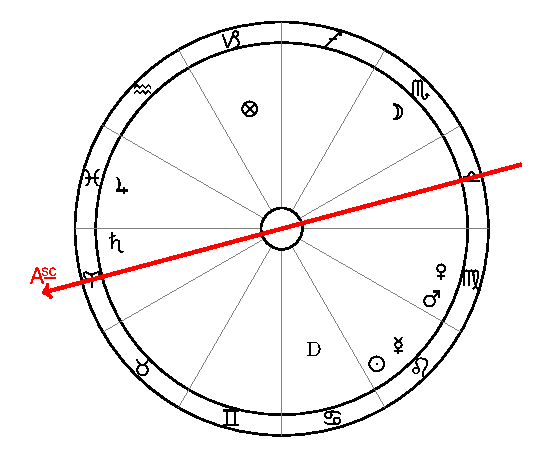
\includegraphics[width=0.68\textwidth]{charts/2_36_11}
\caption{Chart 30 [II.36.11, GH L112]}
\label{fig:chart30}
\end{wrapfigure}


The native was a hunchback.

\newpage